%%%%%%%%%%%%%%%%%%%%%%%%%%%%%%%%%%%%%%%%%%%%%%%%%%%%%%%%%%%%%%%%%%%%%%%%%%%%%%%
% intro.tex: Introduction to the thesis
%%%%%%%%%%%%%%%%%%%%%%%%%%%%%%%%%%%%%%%%%%%%%%%%%%%%%%%%%%%%%%%%%%%%%%%%%%%%%%%%
\chapter{Introduction} \label{chap:intro}
\label{intro_chapter}
%%%%%%%%%%%%%%%%%%%%%%%%%%%%%%%%%%%%%%%%%%%%%%%%%%%%%%%%%%%%%%%%%%%%%%%%%%%%%%%%
A \textit{$G$-decomposition} of a graph $K$ is a set of mutually edge-disjoint subgraphs of $K$ which are isomorphic to a given graph $G$. If such a set exists we say that $K$ \textit{allows} a $G$-decomposition, and if $K\cong K_{n}$ we sometimes call the decomposition a \textit{$G$-design of order $n$}.

$G$-decompositions are a longstanding topic in combinatorics, graph theory, and design theory, with roots tracing back to at least the 19th century. The work of Rosa and Kotzig in the 1960s on what are now known as graph labelings laid the foundation for the modern treatment of such problems. Using adaptations of these labelings alongside techniques from design theory, numerous papers have since been published on $G$-decompositions. This work is a natural continuation of Freyberg and Peters' recent paper on decomposing complete graphs into forests with six edges \cite{bib:Peters}. Their paper also includes a summary of $G$-decompositions for graphs $G$ with less than 7 edges.

Every connected component of a forest with 7 edges is a tree with 6 or less edges. All such trees are cataloged in Figure \ref{fig:catalog}. We use the naming convention $\mathbf{T_{j}^i}$ to denote the $i^{\textrm{th}}$ tree with $j$ vertices. For each tree $\mathbf{T_{j}^i}$, the names of the vertices, $v_t$ for $1 \leq t \leq j,$ will be referred to in the decompositions presented in the main results of this project.

\begin{figure}[H]
\begin{center}
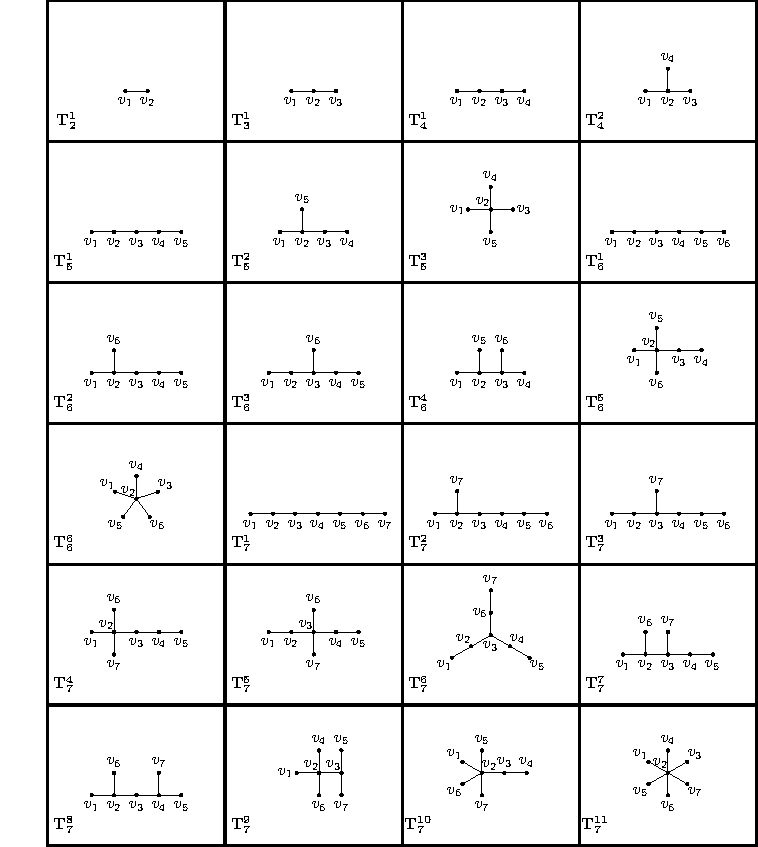
\includegraphics{standalone/tree chart.pdf}
\end{center}
\caption{trees with less than seven edges}
\label{fig:catalog}
\end{figure}

The next theorem gives the necessary conditions for the existence of a $G$-decomposition of $K_n$ when $G$ is a graph with 7 edges.

\begin{thm}

  If $G$ is a graph with $7$ edges and a $G$-decomposition of $K_n$ exists, then $n \equiv 0,1,7, \textrm{or} \; 8 \pmod{14}.$

\end{thm}

\begin{proof}

    If a $G$-decomposition exists, then $7|\binom{n}{2}$ which immediately implies $n \equiv 0,1,7, \textrm{or} \; 8 \pmod{14}.$

\end{proof}

In this article, we only consider simple graphs without isolated vertices. There are $47$ non-isomorphic forests with $7$ edges. Chapter \ref{chap:0,1(mod 14)} treats all $47$ forests when $n \equiv 0 \textrm{ or } 1 \pmod{14}$. Chapter \ref{chap:7,8 (mod 14)} applies to all the forests when $n \equiv 7 \textrm{ or } 8 \pmod{14}$ with the lone exception of $F \cong \mathbf{T_{7}^{11}}\sqcup\mathbf{T_{2}^{1}},$ which is solved for those values of $n$ in Chapter \ref{chap:special case}. 

%\begin{itemize}

%\item Chapter 1 introduces the analytic goals pursued in this thesis.

%\item Chapter 2 briefly presents the history of, and science behind, the
%subjects presented in this thesis.

%\item In Chapter 3 the experiment is outlined.

%\item Chapter 4 describes the simulation process used in the analysis.

%\item Chapter 5 follows the chain of reconstruction software used to obtain
%meaningful results from data.

%\item Chapter 6 hashes out the strategy for analysis and presents the data and
%simulated sets that will be used in the analysis.

%\item Chapter 7 demonstrates the implementation of the event selection
%processes.

%\item In Chapter 8 those events selected in Chapter 7 are analyzed.

%\item Chapter 9 presents a final discussion of the analyses presented in the
%thesis.

%\end{itemize}
%%%%%%%%%%%%%%%%%%%%%%%%%%%%%%%%%%%%%%%%%%%%%%%%%%%%%%%%%%%%%%%%%%%%%%%%%%%%%%%%
